\documentclass[conference]{IEEEtran}
%\IEEEoverridecommandlockouts
% The preceding line is only needed to identify funding in the first footnote. If that is unneeded, please comment it out.
\usepackage{cite}
\usepackage{amsmath,amssymb,amsfonts}
\usepackage{algorithmic}
\usepackage{graphicx}
\usepackage{textcomp}
\usepackage{xcolor}
\usepackage{graphicx}
\usepackage{caption}
\usepackage{subcaption}
\usepackage{hyperref}
\def\BibTeX{{\rm B\kern-.05em{\sc i\kern-.025em b}\kern-.08em
    T\kern-.1667em\lower.7ex\hbox{E}\kern-.125emX}}
\begin{document}

\title{A Unity-Based Pipeline for Multi-View Dataset Generation and 3D Reconstruction Evaluation\\}


\author{\IEEEauthorblockN{Valeria Itrat Herrera}
\IEEEauthorblockA{\textit{Department of Electrical and Computer Engineering} \\
\textit{Rice University}\\
Houston, TX, USA \\
vi6@rice.edu}
}


\maketitle

\begin{abstract}
Recent advances in 3D reconstruction methods, such as Gaussian Splatting, have demonstrated high-quality rendering from multi-view imagery. However, evaluating these methods remains challenging due to the limited availability of datasets with controlled camera configurations and reliable ground truth.

This work presents a Unity-based pipeline for generating synthetic datasets under controlled conditions, enabling configurable camera rigs, synchronized multi-camera capture, and flexible scene setup. Two dataset configurations based on temporal and spatial sampling of viewpoints are evaluated, showing that reconstruction quality strongly depends on viewpoint density and coverage.

A calibration pipeline based on OpenCV is implemented and validated against simulation ground truth and real-world measurements, demonstrating accurate pose estimation. A discrepancy observed when replicating the real setup in simulation highlights the importance of image-space resolution for reliable calibration.

These results demonstrate the potential of simulation as a fast experimentation platform while exposing key challenges in bridging simulated and real-world systems.
\end{abstract}

\begin{IEEEkeywords}
Multi-View, Camera rig, Unity Simulation, 3D reconstruction, Gaussian Splatting
\end{IEEEkeywords}

\section{Introduction}
In recent years, significant advances have been made in computer vision; however, most modern approaches require large amounts of data for training and evaluation. For this reason, many research efforts have explored the use of simulation platforms such as Unity and NVIDIA Omniverse to generate synthetic datasets that can support the development, training, and evaluation of computer vision models \cite{unitySynthetic,synthetic}.

Among the areas that have evolved considerably, 3D reconstruction has received particular attention \cite{overview}. Acquiring datasets for 3D reconstruction is especially challenging, since these methods require reliable ground truth for evaluation and multi-view image datasets captured with synchronized cameras. Recent efforts, such as those developed by Dolby Laboratories, have demonstrated the potential of simulated environments for generating multi-view datasets \cite{volucapture}.

This work presents an open-source Unity-based platform for generating synthetic multi-camera datasets and evaluating 3D reconstruction algorithms, such as Gaussian Splatting \cite{3dgs}. 

The proposed framework enables the creation of configurable camera rigs, synchronized multi-view data capture, and controlled acquisition conditions for experimentation.

This stage of the project focuses on three main aspects: (1) validating the synchronization of the multi-camera capture pipeline, (2) evaluating the accuracy of simulated camera calibration against ground-truth parameters and real-world measurements, and (3) analyzing the impact of different viewpoint sampling strategies on reconstruction performance.

In addition, a comparison between simulated and real-world calibration setups is performed, revealing discrepancies related to the resolution of the calibration target. These findings provide insight into the challenges of bridging simulation and real-world systems and establish a foundation for further development toward a simulation framework that more closely approximates real-world behavior.

The implementation of the proposed framework is available at
\href{https://rice-exp-lab.github.io/universal-reconstruction-simulator/}{https://rice-exp-lab.github.io/universal-reconstruction-simulator/}.

% -------------------------------------------------------- %

\section{Methods}

The system is implemented in Unity, enabling flexible configuration of camera rigs, capture parameters, and calibration setups.

The platform supports two main operational modes. The first mode enables dataset generation by capturing images from simulated camera rigs for 3D reconstruction tasks. The second mode enables camera calibration using a ChArUco board and the OpenCV library.

\subsection{Simulated Environment}

The project is developed using the Unity High Definition Render Pipeline (HDRP), which provides advanced rendering capabilities, including physically-based lighting and camera effects.

The simulated environment represents an indoor laboratory scene where a multi-camera system would be deployed in practice (Figure \ref{fig:lab}). The scene includes configurable lighting conditions and camera effects to emulate realistic acquisition scenarios.

A camera rig generation script allows users to automatically create camera arrays around a target object. The user specifies the number of cameras, their heights, radial distances from the object, and angular distribution. The cameras are then placed evenly around the object to simulate typical multi-view capture configurations.

\begin{figure}[ht] 
\centering 
\begin{subfigure}[b]{0.3\textwidth} 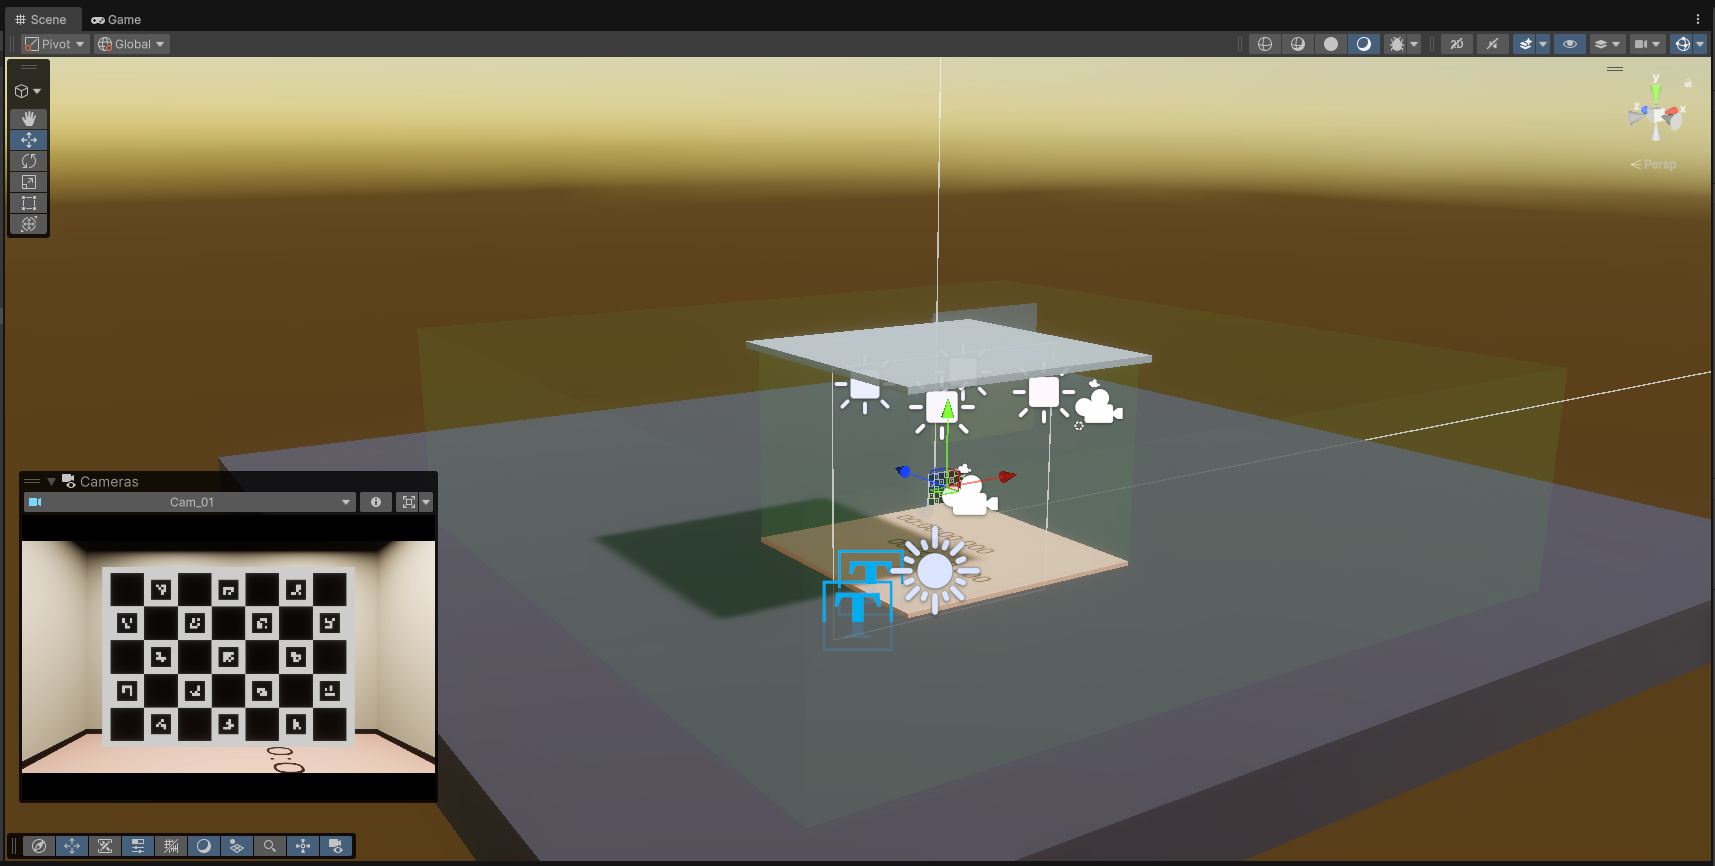
\includegraphics[width=\textwidth]{images/lab_no_wall.png} \caption{Lab building} 
\end{subfigure} 
\hfill 
\begin{subfigure}[b]{0.3\textwidth} 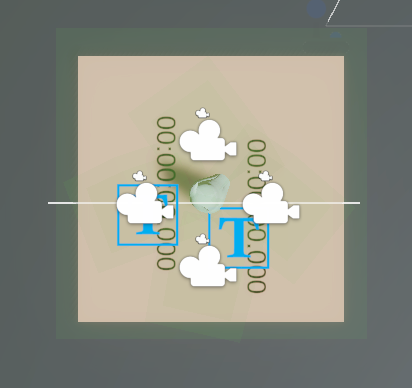
\includegraphics[width=\textwidth]{images/lab_in_top2.png} \caption{Multiple camera setup} 
\end{subfigure} 
\caption{Simulated laboratory environment in Unity.} \label{fig:lab} 
\end{figure}

To increase the variety of viewpoints and capture conditions, camera motion can be introduced during acquisition. The system supports different motion patterns, including linear translation and circular or spiral trajectories around the target object.

\subsection{Camera Modeling}
The simulated cameras are configured using Unity’s Physical Camera model. The camera parameters are based on the specifications of the Azure Kinect DK camera, which will be used in the real-world setup.

The camera model includes parameters such as sensor size, focal length, and field of view. %Additionally, Unity’s HDRP local volumes support optical effects, such as depth of field and lens distortion, enabling experimentation with different imaging conditions.%

\begin{itemize}
    \item Sensor size: $5.120 \times 3.132$
    \item Horizontal field of view: $90^\circ$
    \item Aperture: $f/2.2$
\end{itemize}


\subsection{Dataset Generation}
The platform allows users to generate synthetic datasets by capturing frames from the simulated cameras.

Capture parameters, such as image resolution, frame rate, and the total number of frames, can be configured by the user prior to acquisition. 

To verify the timing accuracy of the capture process and ensure proper synchronization when multiple cameras are used, a digital timer object that displays timestamps with millisecond precision is placed in the scene and recorded in the captured frames.

\subsection{3D Gaussian Splatting Reconstruction}

For reconstruction experiments, the official implementation of 3D Gaussian Splatting provided by INRIA was used \cite{gaussian-splatting}.

Two datasets were generated. The first dataset was obtained by moving a single camera along a spiral trajectory around a static object, producing 225 images at 15 frames per second. This setup provides dense temporal sampling of viewpoints.

The second dataset was generated using 40 cameras positioned around the object, capturing one image per camera simultaneously, resulting in 40 images. This setup provides spatial sampling of viewpoints.

While both datasets consist of multiple images, they differ in how viewpoints are sampled: temporally in the single-camera case and spatially in the multi-camera case. In this work, it is refer to the first as a multi-frame dataset and the second as a multi-view dataset. 

The overall dataset generation and reconstruction workflow is shown in Fig.~\ref{fig:pipeline}.

 \begin{figure}[htbp]
    \centering
    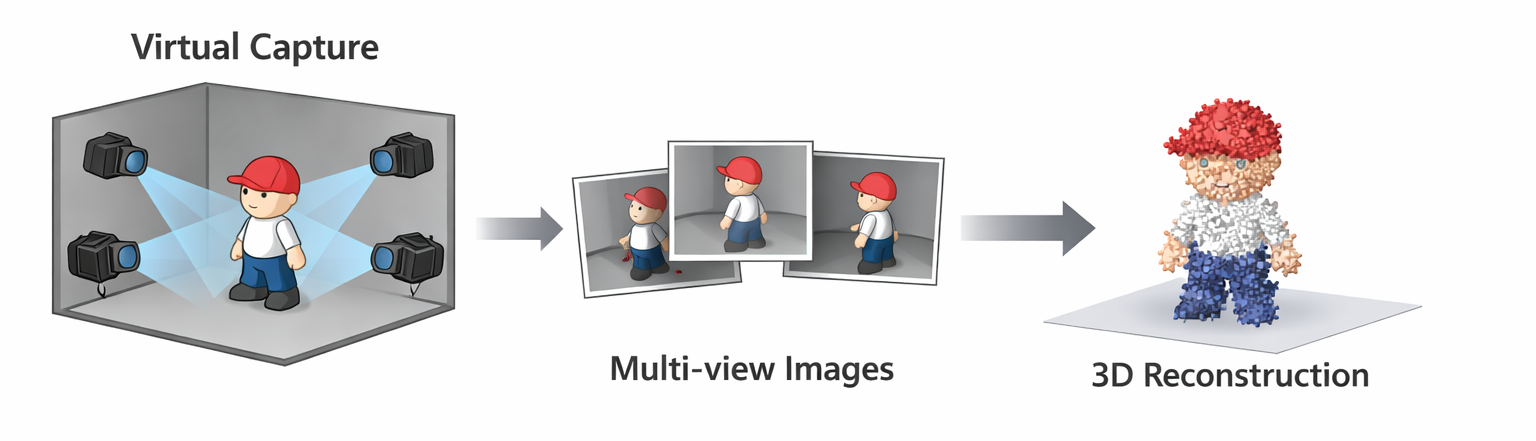
\includegraphics[width=\linewidth]{images/multi_view.png}
    \caption{Multi-view dataset application pipeline}
    \label{fig:pipeline}
\end{figure}

For the multi-frame dataset, two capture configurations were tested. In the first experiment, the camera completed three full rotations around the object during the capture interval. In the second configuration, the camera performed two rotations over the same duration, resulting in slower motion and improved view coverage.

The second configuration produced significantly better reconstruction results, while the first failed to recover the full geometry of the object.

\subsection{Camera Calibration}

\subsubsection{Calibration pipeline in Unity}
To estimate the intrinsic and extrinsic parameters of the simulated camera, a calibration pipeline based on OpenCV for Unity was implemented \cite{openCV}.

A ChArUco calibration board is generated in the Unity scene using configurable parameters, including the number and size of squares, the marker size, and the dictionary type.

During calibration mode, markers and board corners are detected in the captured frames using OpenCV’s ArUco detection algorithms and displayed in the preview view. 
The user captures multiple frames as they move the board to different positions and orientations to obtain a diverse set of observations. Once a sufficient number of frames have been collected, the calibration procedure is executed to estimate the intrinsic camera matrix and the extrinsic parameters relative to the calibration board.

These estimated parameters are later compared with the ground-truth camera parameters available from the Unity simulation. 

%The calibration pipeline implemented in the system is illustrated in Figure \ref{fig:calibration}.

% \begin{figure}[htbp]
%    \centering
%    \includegraphics[width=\linewidth]%{images/calibration.png}
%    \caption{Calibration pipeline}
%    \label{fig:calibration}
%\end{figure}

\subsubsection{Calibration in Real-World}
To validate the simulated camera models, a stereo calibration setup was implemented in the laboratory.

Two cameras were placed with a baseline of 1.50 m, oriented toward a Charuco board (Fig.~\ref{fig:geometry}). The distance from each camera to the board was approximately 1.65 m, and the board was mounted at a height of 1.16 m.

The board was rotated around the three axes to known angles, providing a diverse set of observations for calibration.


\begin{figure}
    \centering
    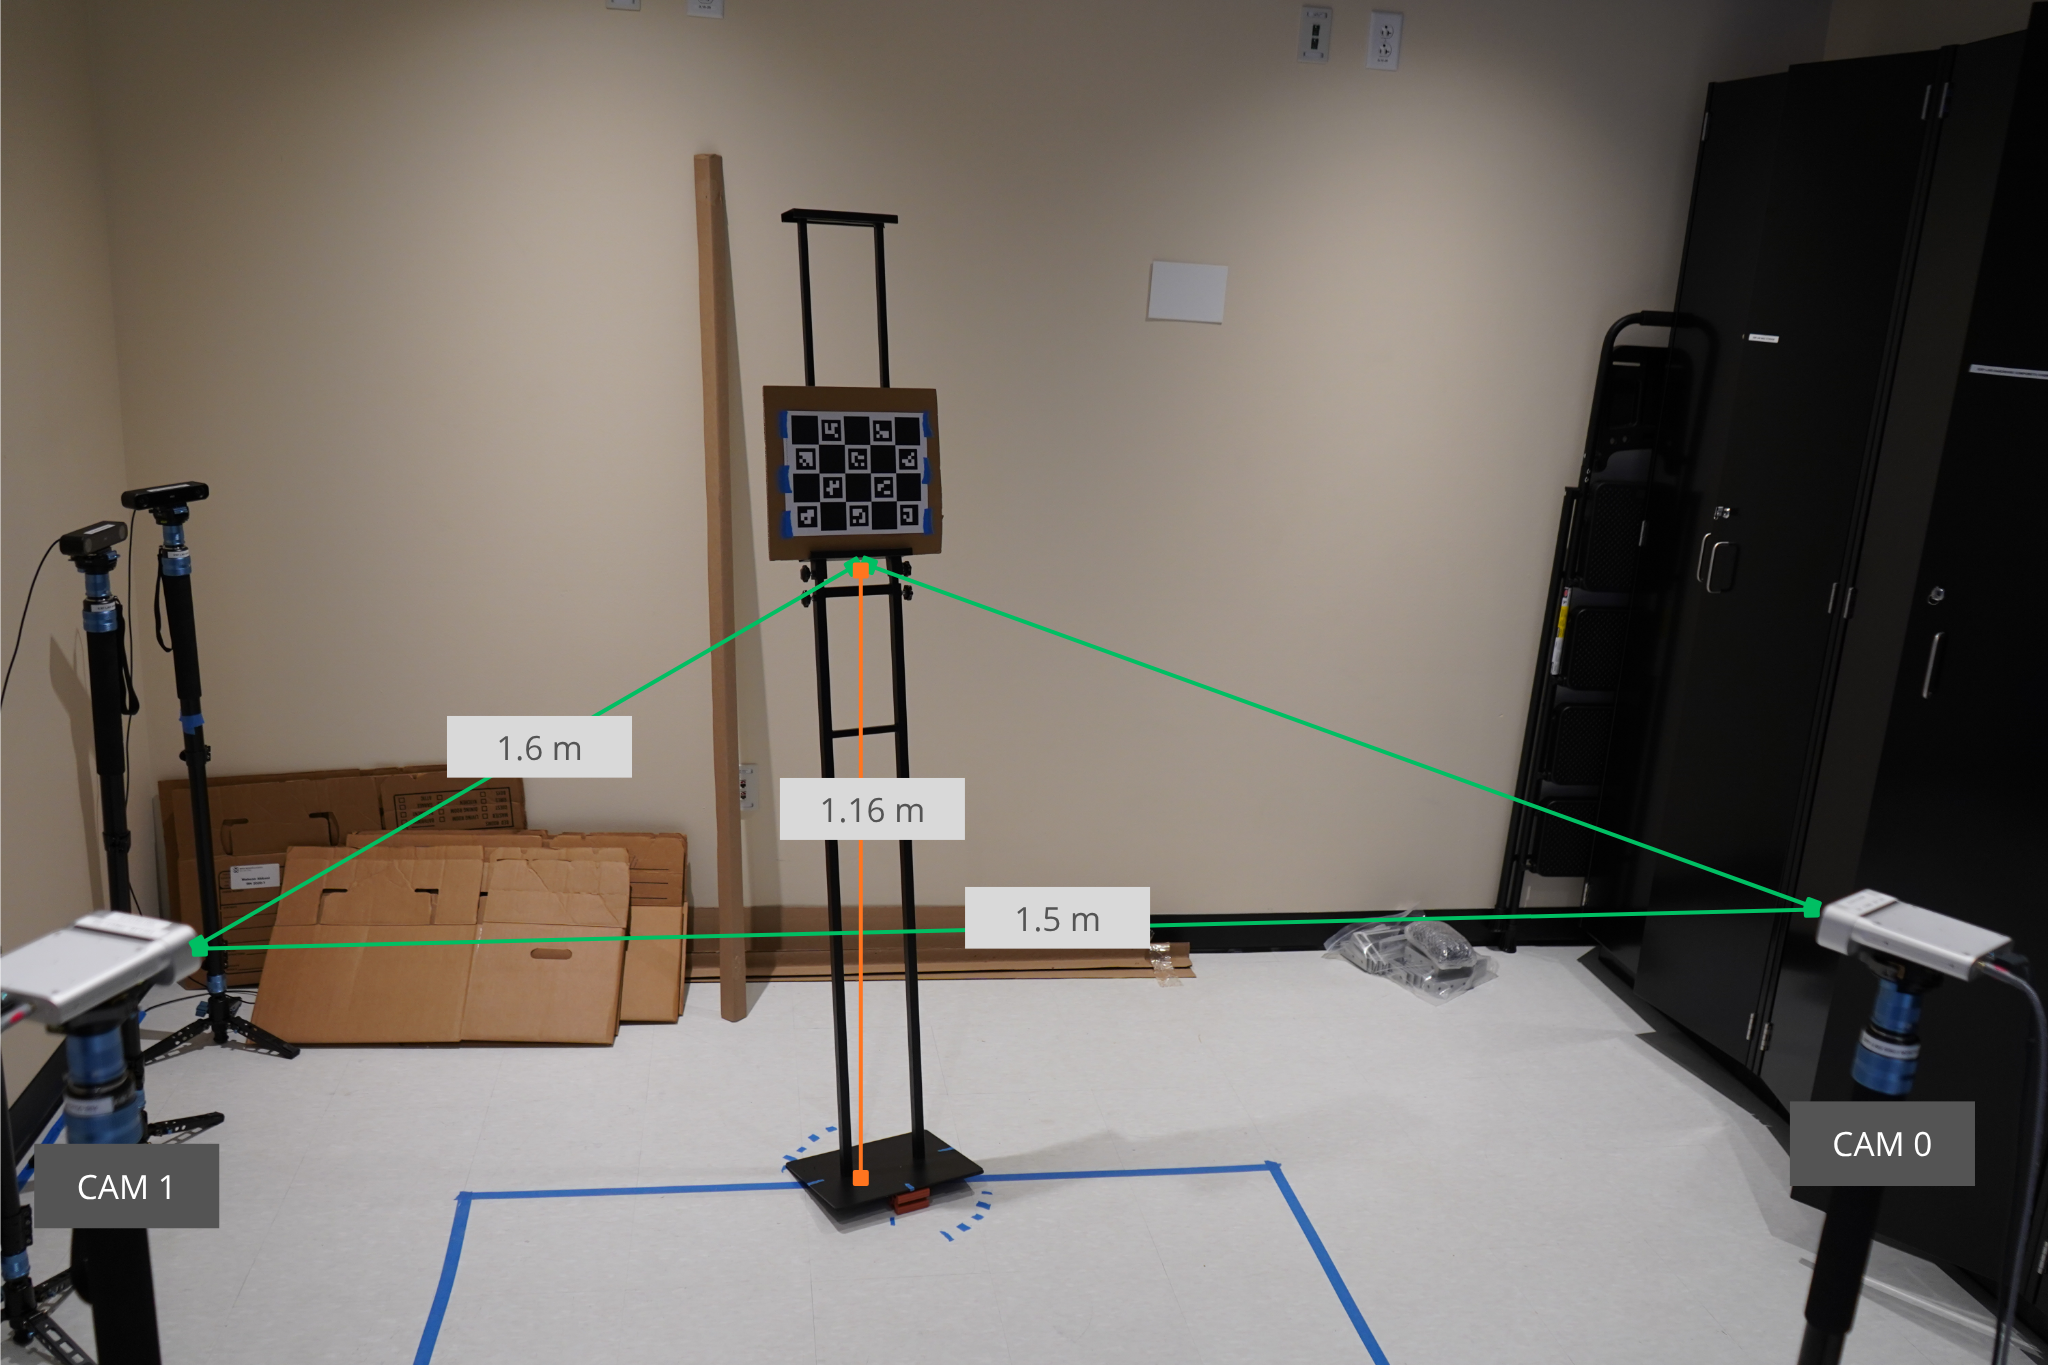
\includegraphics[width=\linewidth]{images/geometry.png}
    \caption{Stereo geometry real-world setup}
    \label{fig:geometry}
\end{figure}

Later, this same geometry and board dimensions were replicated in the Unity simulator to run the calibration, moving the camera in the same angles, and comparing the behavior of the real camera and the simulated model. 

% -------------------------------------------------------- %
\section{Results}

\subsection{Dataset}

To evaluate the synchronization of the camera rig when working with multiple cameras, four cameras were placed around the target object in the scene, each following different motion trajectories at 15 FPS. Frames captured by different cameras at the same time step share matching timestamps, and the corresponding entries in the dataset metadata reflect the same acquisition time.

To further verify the synchronization of the capture process, a digital clock displaying time with millisecond precision was placed on the floor of the scene. The clock is visible from all camera views (Figure \ref{fig:sync}), allowing direct visual confirmation that frames captured at the same timestep correspond to the same timestamp across the different cameras.

This confirms that the capture pipeline maintains correct synchronization across the camera rig.

 \begin{figure}[htbp]
    \centering
    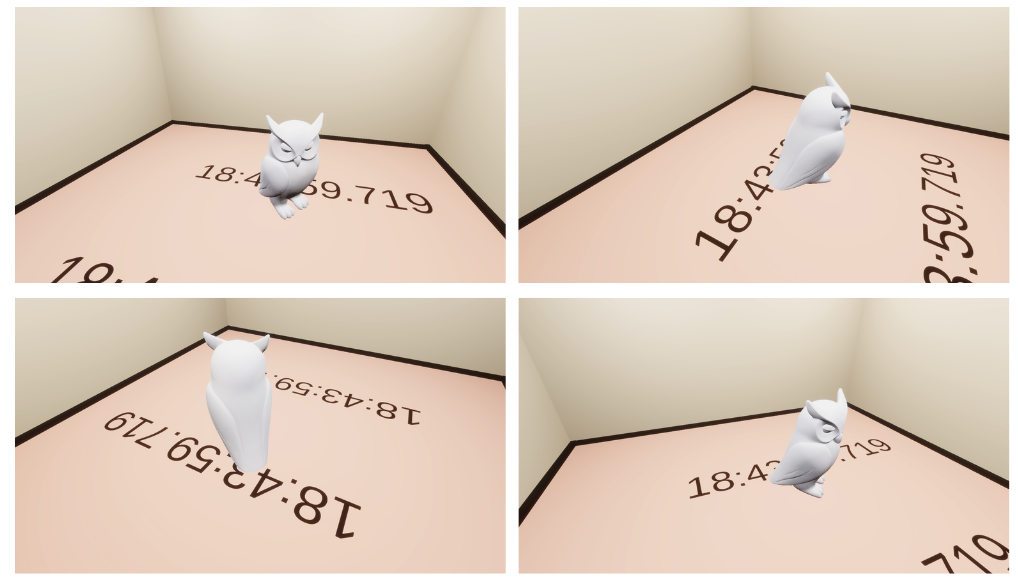
\includegraphics[width=\linewidth]{images/sync.png}
    \caption{Multi-camera synchronization validation. Frames captured at the same timestep share identical timestamps across different camera views.}
    \label{fig:sync}
\end{figure}


\subsection{3D Gaussian Splatting Reconstruction}

The reconstruction results obtained from the temporally sampled dataset are promising. The quantitative metrics computed on the training dataset are shown in Table~\ref{tab:results}. These results indicate that the model successfully converged and that the reconstruction provides a good approximation of the scene geometry and appearance (Fig.~\ref{fig:3dgs}).

 \begin{figure}[htbp]
    \centering
    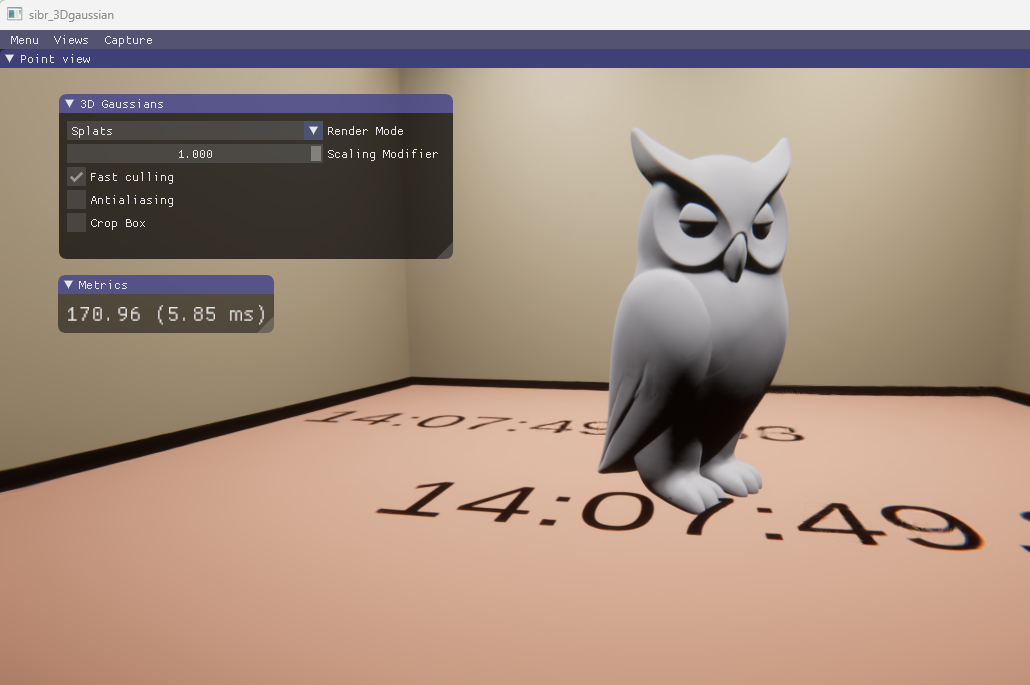
\includegraphics[width=\linewidth]{images/3dgs.png}
    \caption{3D Gaussian Splatting reconstruction from the temporally sampled dataset, showing accurate geometry and appearance recovery.}
    \label{fig:3dgs}
\end{figure}

A visualization of the reconstruction can be seen in the video available at \href{https://youtu.be/-RY_b5SnkdY}{https://youtu.be/-RY\_b5SnkdY}.

In contrast, the reconstruction obtained from the spatially sampled dataset exhibited lower quality, as shown in Fig.~\ref{fig:out_multi}.

The difference in reconstruction quality between both datasets can be explained by the density and distribution of viewpoints.

In the temporally sampled dataset, the camera motion provides a dense and continuous coverage of the scene, allowing the reconstruction algorithm to observe the object from multiple overlapping perspectives. This results in improved geometric consistency and more stable splat estimation.

In contrast, the spatially sampled dataset contains a limited number of viewpoints, which reduces overlap between observations and leads to incomplete geometry reconstruction. This effect is particularly noticeable when inspecting the reconstructed model at close range, where instability and missing structure can be observed.

These results suggest that, for methods such as Gaussian Splatting, viewpoint density and coverage play a critical role in reconstruction quality, even when using a true multi-camera setup.

\begin{figure}
    \centering
    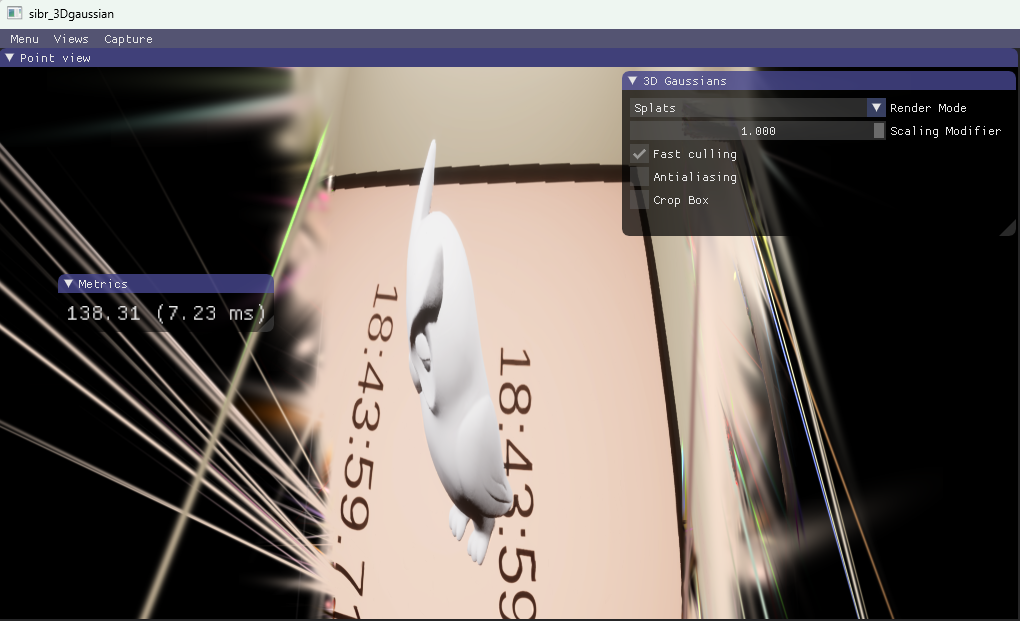
\includegraphics[width=\linewidth]{images/output_multicam.png}
    \caption{3D Gaussian Splatting reconstruction from the spatially sampled dataset, showing incomplete geometry and reduced stability due to limited viewpoint coverage.}
    \label{fig:out_multi}
\end{figure}

These results highlight the importance of viewpoint density and coverage in 3D reconstruction performance. 

They also demonstrate the value of simulation as a fast experimentation platform. By testing different camera configurations in Unity, it is possible to rapidly evaluate how factors such as view count and spatial distribution affect reconstruction quality before implementing a physical setup.

Future work will focus on improving multi-view camera configurations to achieve results closer to the temporally sampled dataset, for example by increasing the number of cameras or introducing additional viewpoints at different heights and angles.

\begin{table}[htbp]
\caption{3DGS Reconstruction Metrics (Temporally Sampled Dataset)}
\label{tab:results}
\centering
\begin{tabular}{|c|c|}
\hline
\textbf{Metric} & \textbf{Result} \\
\hline
PSNR (dB) & 30.99 \\
SSIM & 0.986 \\
LPIPS & 0.029 \\
\hline
\end{tabular}
\end{table}

\subsection{Camera Calibration}
\subsubsection{Calibration in Unity}
%The intrinsic camera matrix estimated using the OpenCV calibration pipeline is

%\begin{equation}
%K =
%\begin{bmatrix}
%761.65 & 0 & 639.87 \\
%0 & 761.67 & 359.50 \\
%0 & 0 & 1
%\end{bmatrix}
%\end{equation}

The reprojection root mean square (RMS) error of the calibration is 0.153 pixels. The focal length values $(f_x, f_y)$ are nearly identical, which is consistent with the expected behavior of the camera model. In addition, the estimated principal point $(c_x, c_y)$ is close to the center of the image resolution (1280×720), indicating that the intrinsic parameters are consistent with the simulated camera configuration.

%The rotation matrix estimated by OpenCV is

%\begin{equation}
%R =
%\begin{bmatrix}
%0.99224 & 0.12435 & -1.74\times10^{-5} \\
%-0.12343 & 0.98488 & -0.12157 \\
%-0.01510 & 0.12063 & 0.99258
%\end{bmatrix}
%\end{equation}

The estimated rotation was compared with the ground-truth rotation obtained from Unity. The angular difference between the two rotations was approximately $0.0000^\circ$, indicating near-perfect alignment between the estimated pose and the simulated ground truth.

%The translation vector estimated by the OpenCV calibration is

%\begin{equation}
%t =
%\begin{bmatrix}
%-0.343 \\
%-0.196 \\
%0.628
%\end{bmatrix}
%\end{equation}

The translation error between the estimated pose and the Unity ground truth is approximately 1.0 mm.

%\begin{table}[h]
%\centering
%\begin{tabular}{lcc}
%\hline
%Parameter & Error \\
%\hline
%Rotation error & \multicolumn{2}{c}{0.0000°} \\
%Translation error & \multicolumn{2}{c}{1.00 mm} \\
%Re-projection error (RMS) & \multicolumn{2}{c}{0.153} \\
%\hline
%\end{tabular}
%\caption{Comparison between OpenCV calibration and Unity ground-truth.}
%\label{tab:resultsCalib}
%\end{table}

%The results in Table \ref{tab:resultsCalib} 
These results indicate that the calibration pipeline implemented in the simulated environment accurately recovers the camera pose relative to the ChArUco board, achieving millimeter translation accuracy and negligible rotation error.

\subsubsection{Calibration in Real-World}
In the real-world setup, the reprojection errors were 0.055 px for camera 0 and 0.050 px for camera 1, indicating reliable calibration performance.

In addition, the estimated baseline was 1.49 m, closely matching the physical distance between the cameras.

The detected corners (circles) and reprojected points (crosses) are shown on the calibration board in Figure \ref{fig:calib_val}. The close alignment between both indicates an accurate calibration.

\begin{figure}
    \centering
    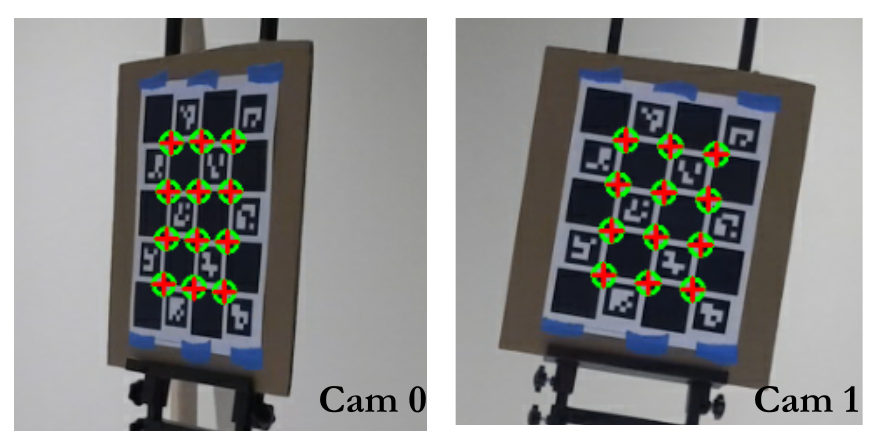
\includegraphics[width=\linewidth]{images/Cam 0.png}
    \caption{Reprojection validation. Detected ChArUco corners (circles) and reprojected points (crosses).}
    \label{fig:calib_val}
\end{figure}



\subsection{Sim-to-Real Analysis}
To further evaluate the simulation framework, the same stereo calibration setup was replicated in Unity using identical geometric parameters (Figure \ref{fig:geoUnity}).

\begin{figure}
    \centering
    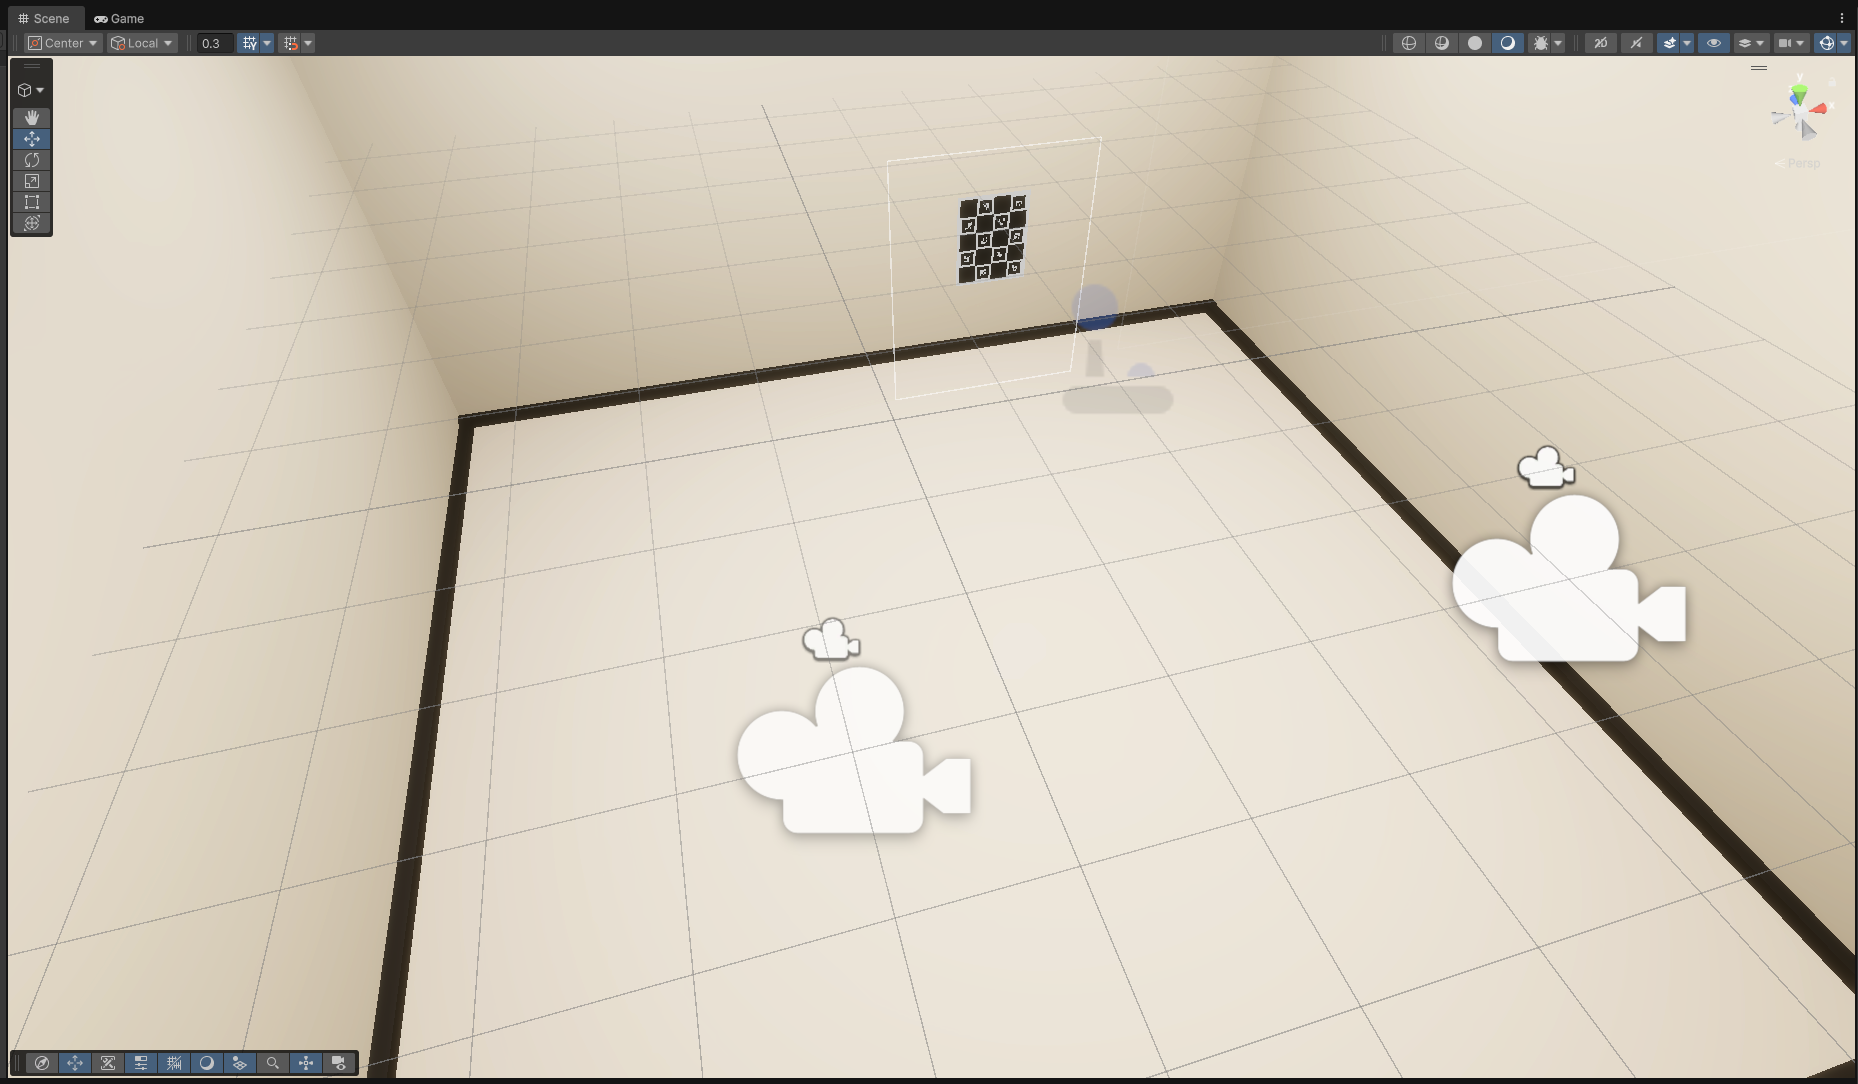
\includegraphics[width=\linewidth]{images/geo_unity.png}
    \caption{Stereo calibration setup replicated in Unity using the same geometric configuration as the real-world experiment.}
    \label{fig:geoUnity}
\end{figure}

While the real-world calibration produced reliable results, a discrepancy was observed in the simulated environment.

Although the physical dimensions matched the real-world setup, the ChArUco board occupied too few pixels in the rendered image for reliable detection, causing the corner detection algorithm to fail.

Initial experiments indicate that increasing the effective board size in the image improves detection stability.

This result shows that matching the physical setup alone is not sufficient for calibration in simulation, as the detectability of the calibration pattern depends on its effective pixel resolution in the rendered image.

This discrepancy highlights an important aspect in the development of simulation-based pipelines, and motivates further investigation into the impact of rendering resolution, camera modeling, and target size on calibration performance.


\section{Discussion}  

The results obtained in this work demonstrate that the proposed simulation pipeline can effectively support controlled experimentation for 3D reconstruction tasks. In particular, the platform enables flexible configuration of camera rigs and synchronized data acquisition, which are difficult to achieve consistently in real-world setups.

The reconstruction experiments highlight the importance of viewpoint density and coverage. The temporally sampled dataset produced significantly better results than the spatially sampled dataset, suggesting that the number and distribution of viewpoints are critical factors for reconstruction quality, even when using a multi-camera configuration.

The calibration experiments further validate the internal consistency of the simulation, showing millimeter-level accuracy and negligible rotation error when compared to Unity ground truth. These results indicate that the calibration pipeline is reliable within the simulated environment.

However, the comparison between the simulated and real-world setups revealed an important discrepancy. While the physical geometry of the setup can be accurately replicated in Unity, successful calibration also depends on the effective image resolution of the calibration target. In the simulated environment, the ChArUco board occupied too few pixels for reliable corner detection, despite matching the real-world dimensions.

Future work will focus on addressing this discrepancy by studying the impact of rendering resolution, camera modeling, and target visibility in the simulated environment. In addition, further experiments will explore improved multi-view camera configurations and evaluate alternative reconstruction methods.

The overall objective is to better understand how simulated camera setups can approximate real-world behavior, moving toward a more accurate and reliable simulation framework for multi-view reconstruction.

\section*{Acknowledgment}
The authors declare no potential conflicts of interest.

The author thanks Prof. Robert LiKamWa and PhD Candidate Krutik Pandya for their guidance and support throughout this project.

\section*{CRediT Author Statement}
Valeria Itrat Herrera: Conceptualization, Methodology, Software, Investigation, Data Curation, Writing - Original Draft, Writing - Review and Editing

\bibliographystyle{IEEEtran}
\bibliography{references}

\end{document}
